During the draft of the alloy, we omitted the aspects regarding the chain of custody because, as mentioned in Security description (3.7.3), these controls are made before storing information in the system, thus the other portions of the application are able to ignore it.

For this reason there is no constraint in Alloy that checks the fact that the report and the image can only exist if the information are genuine.
\subsection{Alloy code}
\begin{figure}
	\centering
	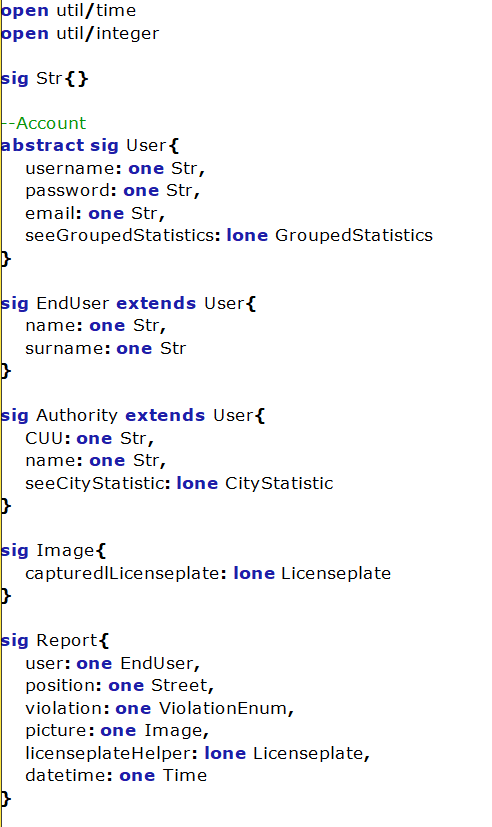
\includegraphics[width=0.9\linewidth, height=0.8 \textheight]{Images/Alloy/codealloy1}
	\caption{Signature 1}
	\label{Signature 1}
\end{figure}

\begin{figure}
	\centering
	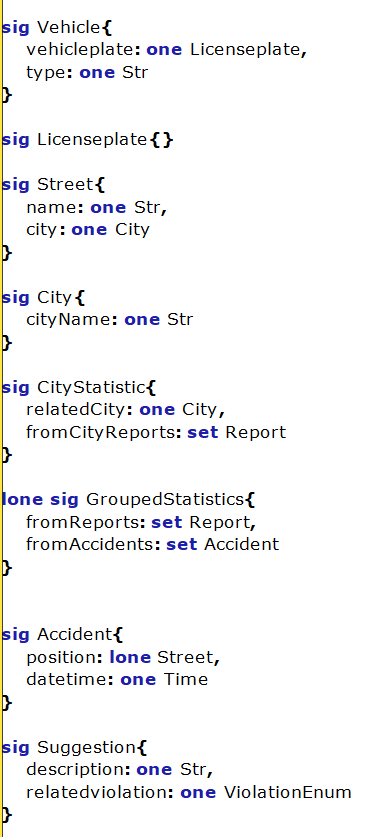
\includegraphics[width=0.7\linewidth, height=0.7\textheight]{Images/Alloy/codealloy2}
	\caption{Signature 2}
	\label{Signature 2}
\end{figure}

\begin{figure}
	\centering
	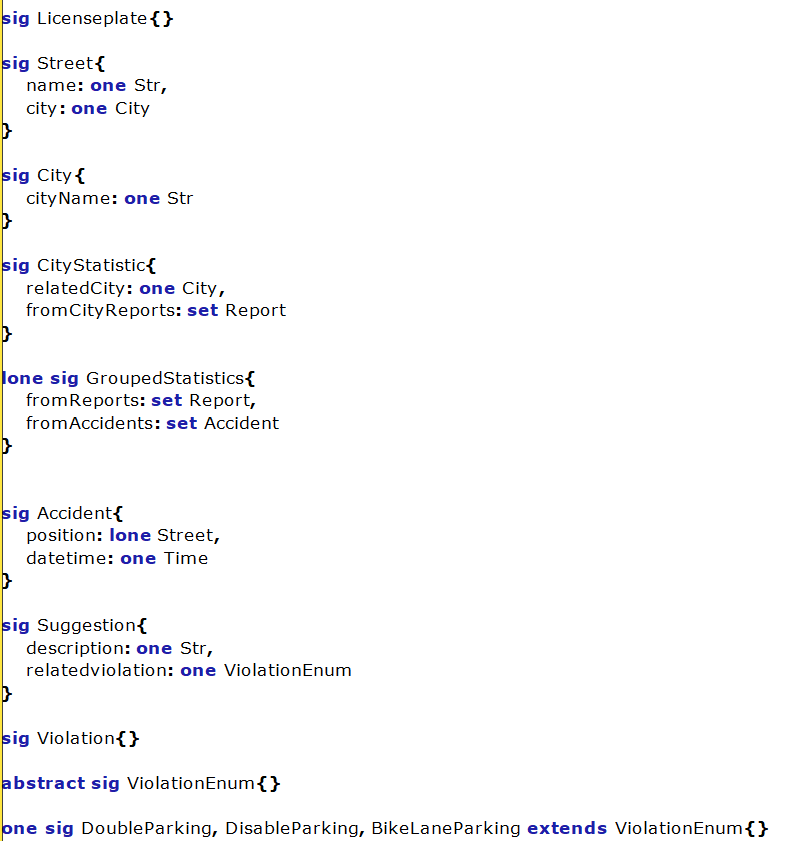
\includegraphics[width=0.9\linewidth, height=0.7\textheight]{Images/Alloy/codealloy3}
	\caption{Signature 3}
	\label{Signature 3}
\end{figure}

\begin{figure}
	\centering
	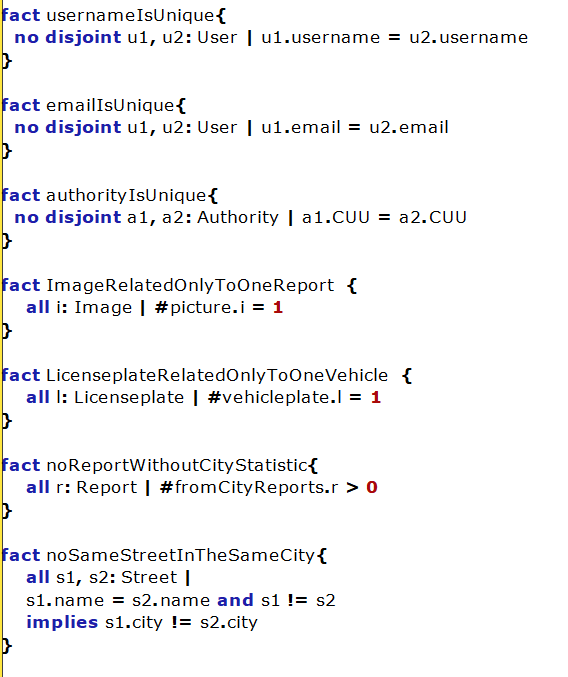
\includegraphics[width=0.9\linewidth, height=0.8\textheight]{Images/Alloy/codealloy4}
	\caption{Pred and Facts 1}
	\label{Pred and Facts 1}
\end{figure}

\begin{figure}
	\centering
	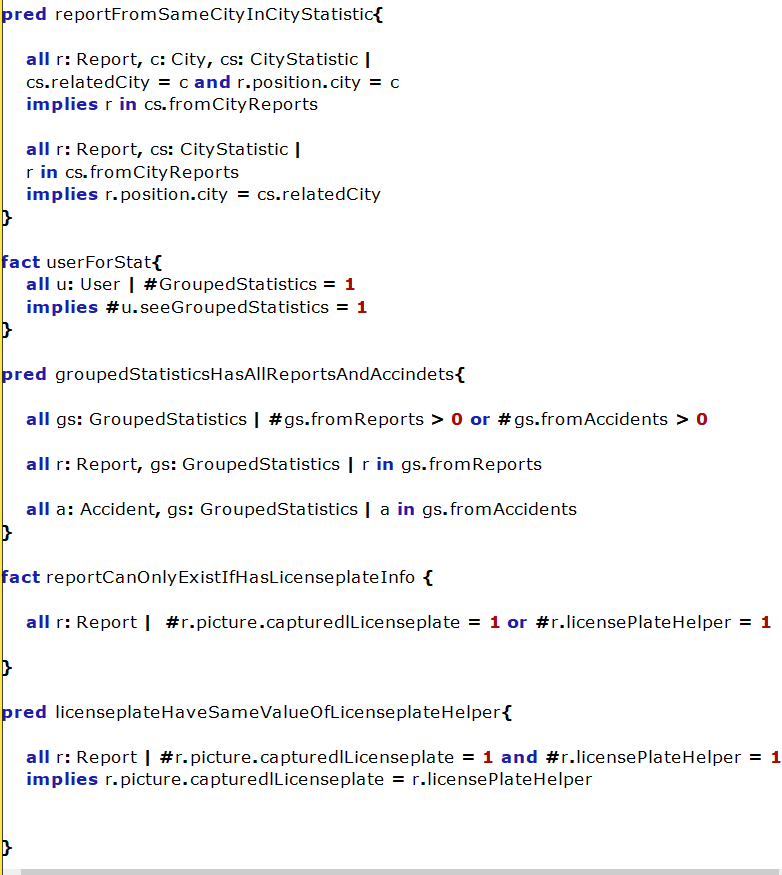
\includegraphics[width=0.9\linewidth, height=0.8\textheight]{Images/Alloy/codealloy5}
	\caption{Pred and Facts 2}
	\label{Pred and Facts 2}
\end{figure}

\begin{figure}
	\centering
	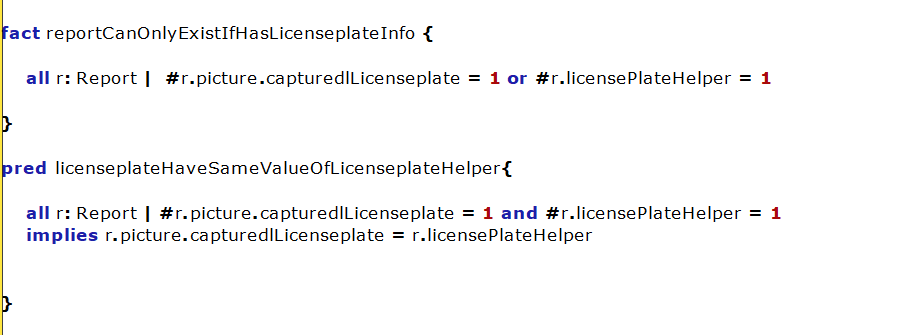
\includegraphics[width=0.9\linewidth, height=0.3\textheight]{Images/Alloy/codealloy6}
	\caption{Pred and Facts 3}
	\label{Pred and Facts 3}
\end{figure}

\begin{figure}
	\centering
	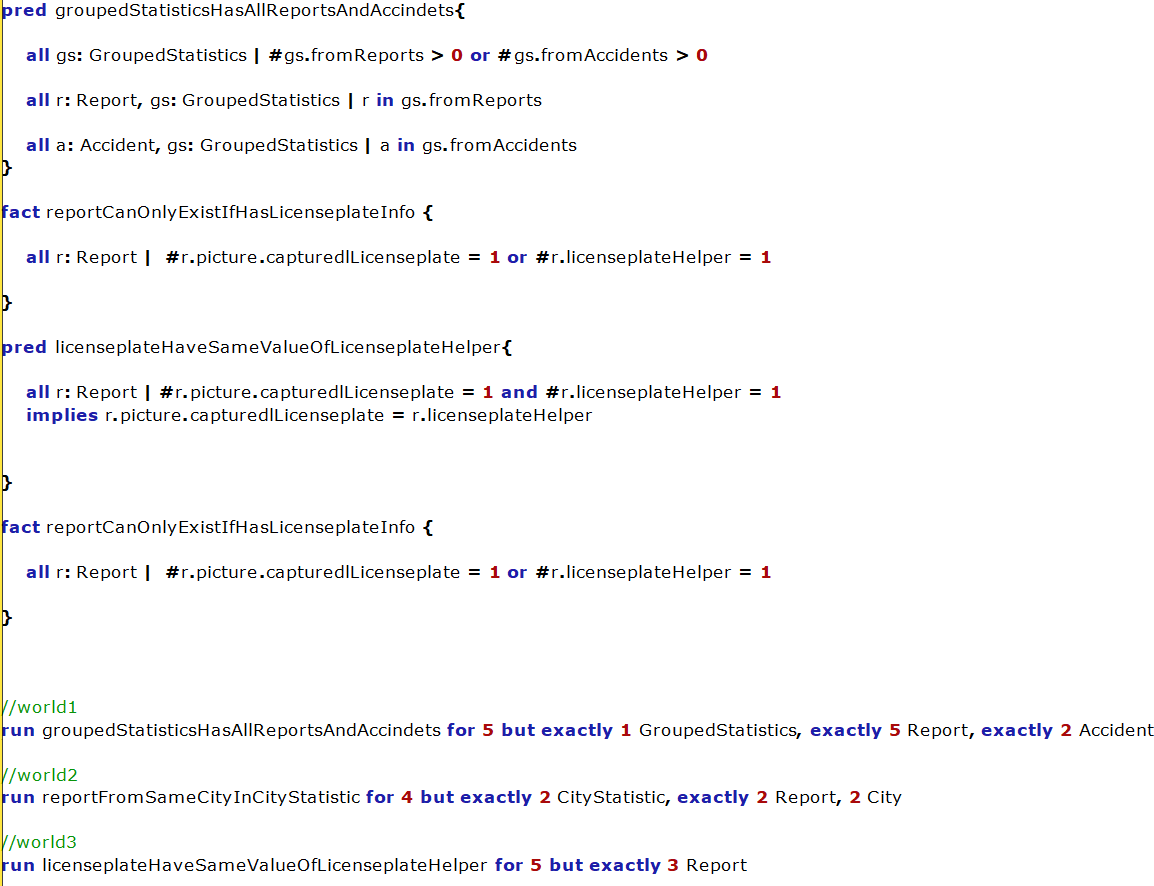
\includegraphics[width=0.95\linewidth, height=0.86\textheight]{Images/Alloy/codealloy7}
	\caption{Pred, Facts and World}
	\label{Pred and Facts and World}
\end{figure}


\subsection{Predicates testing}
\begin{figure}
	\centering
	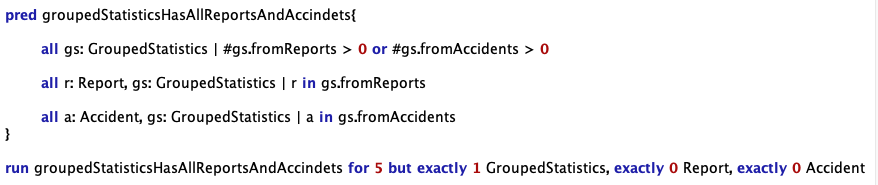
\includegraphics[width=0.9\linewidth, height=0.15\textheight]{Images/Alloy/test-world11}
	\caption{Predicate about the aggregation of data coming from reports with the traffic information.}
	\label{Pred 1}
\end{figure}

\begin{figure}
	\centering
	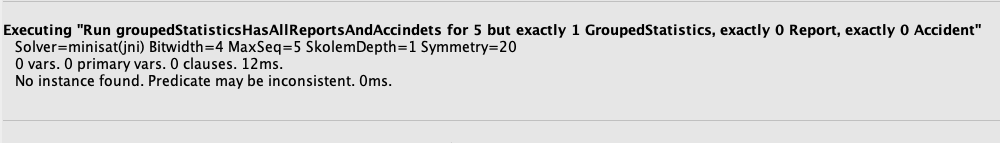
\includegraphics[width=0.9\linewidth, height=0.12\textheight]{Images/Alloy/test-world12}
	\caption{Result pred 1}
	\label{Result pred 1}
\end{figure}

\begin{figure}
	\centering
	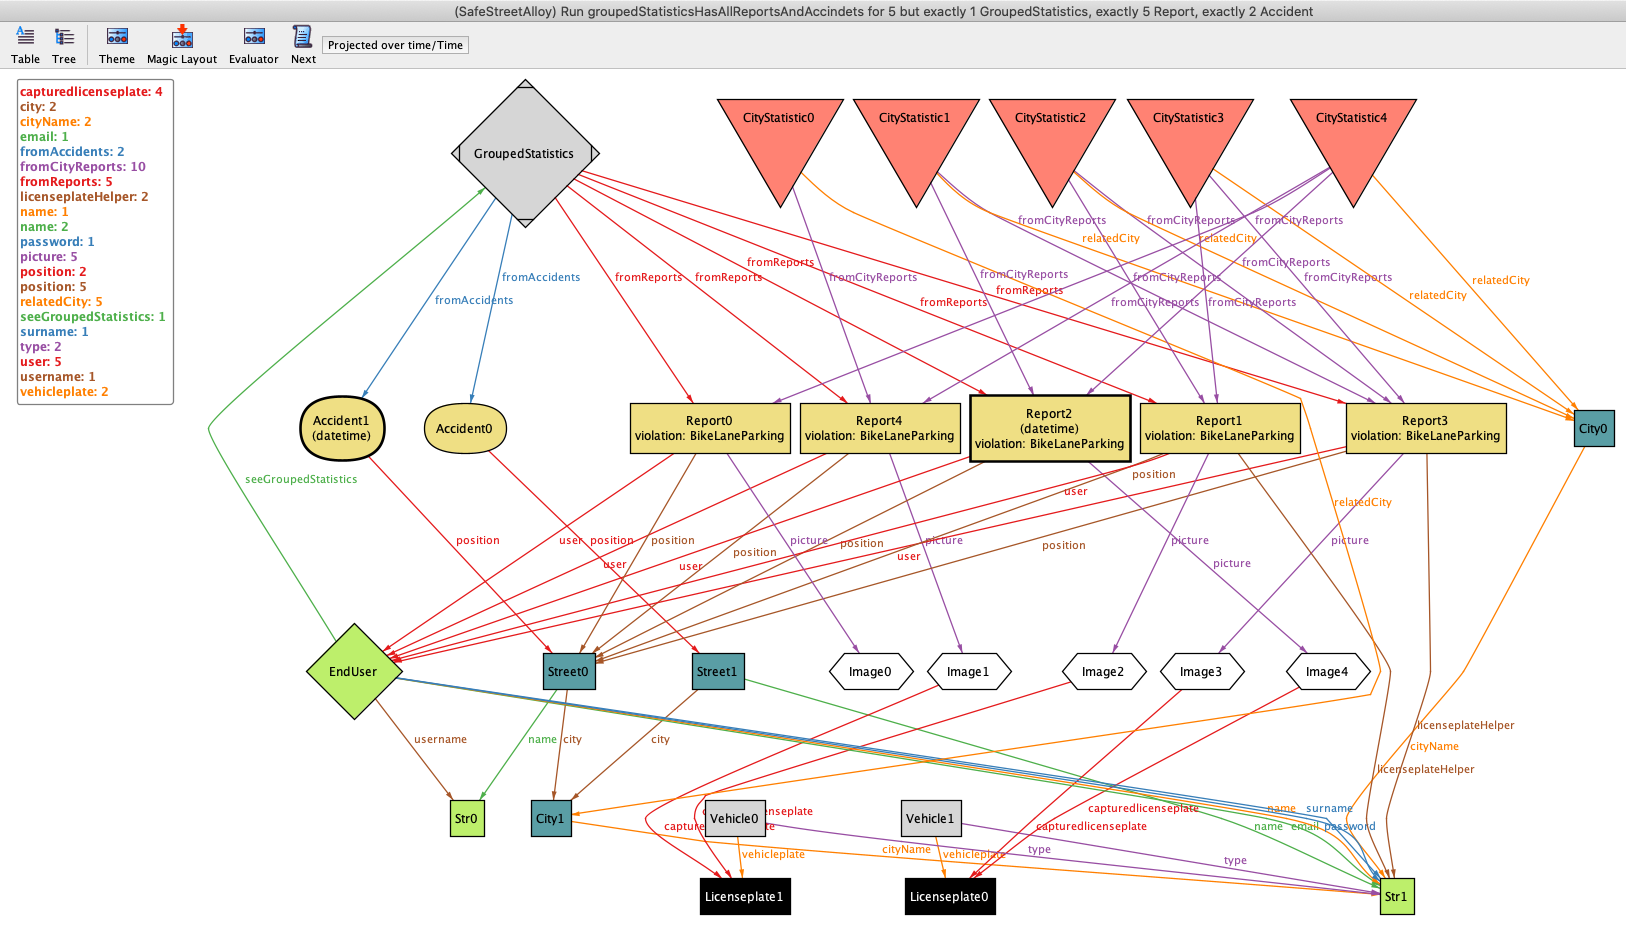
\includegraphics[width=0.9\linewidth, height=0.5\textheight]{Images/Alloy/world1}
	\caption{World 1 generated by pred 1}
	\label{World1 }
\end{figure}
\newpage
\begin{figure}
	\centering
	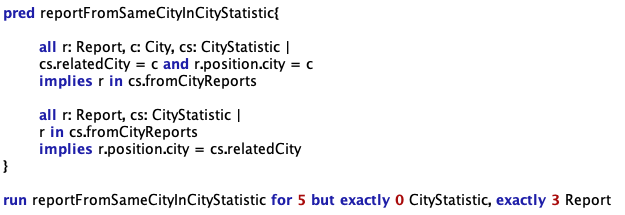
\includegraphics[width=0.9\linewidth, height=0.15\textheight]{Images/Alloy/test-world21}
	\caption{Consistency between city and statistics.}
	\label{Pred 2}
\end{figure}

\begin{figure}
	\centering
	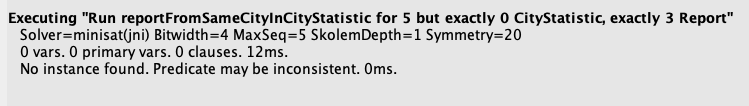
\includegraphics[width=0.9\linewidth, height=0.11\textheight]{Images/Alloy/test-world22}
	\caption{Result pred 2}
	\label{Result pred 2}
\end{figure}

\begin{figure}
	\centering
	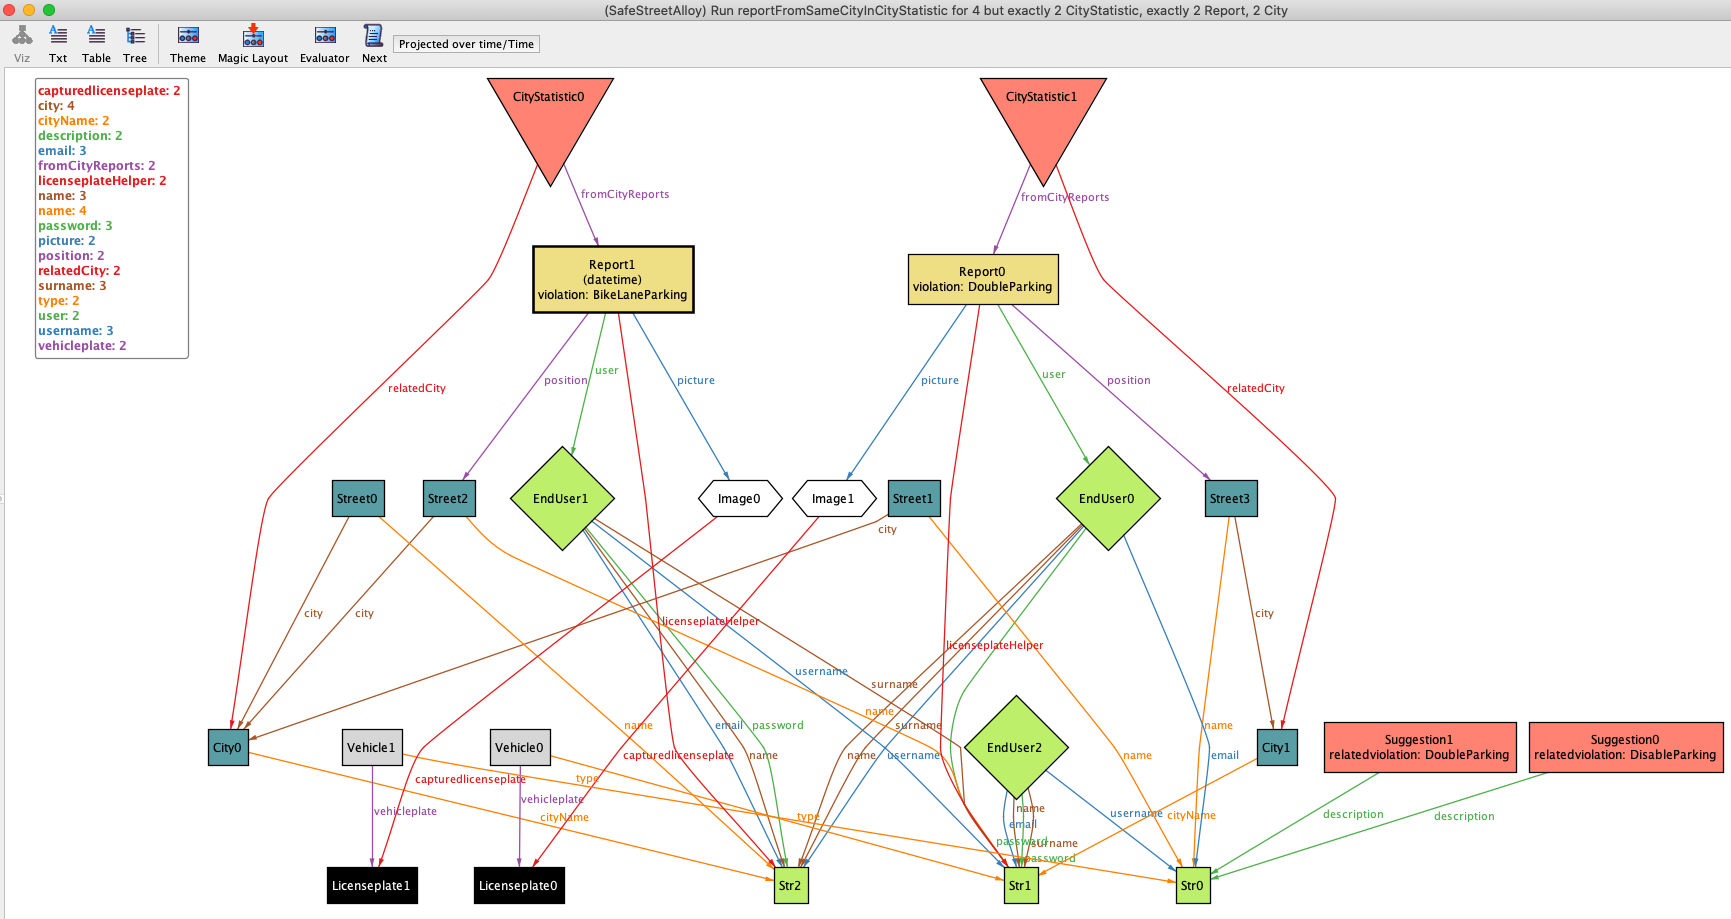
\includegraphics[width=1\linewidth, height=0.47\textheight]{Images/Alloy/world2}
	\caption{World 2}
	\label{World2}
\end{figure}

\begin{figure}
	\centering
	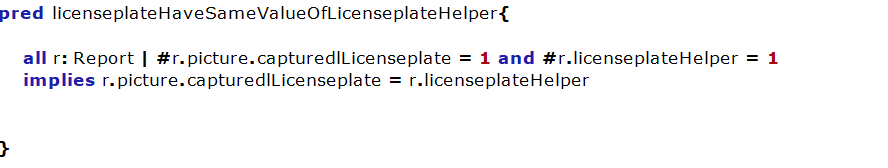
\includegraphics[width=0.9\linewidth, height=0.15\textheight]{Images/Alloy/predworld31}
	\caption{Predicate that test if the licenseplate retrieve from SafeStreets is the same suggested by the user.}
	\label{Pred 3}
\end{figure}

\begin{figure}
	\centering
	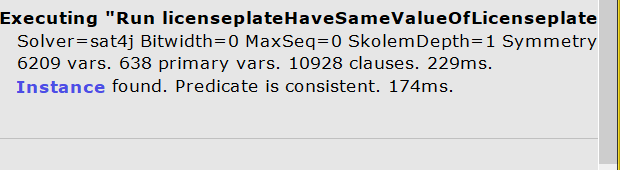
\includegraphics[width=0.8\linewidth, height=0.11\textheight]{Images/Alloy/predworld32}
	\caption{Result pred 3}
	\label{Result pred 3}
\end{figure}


\begin{figure}
	\centering
	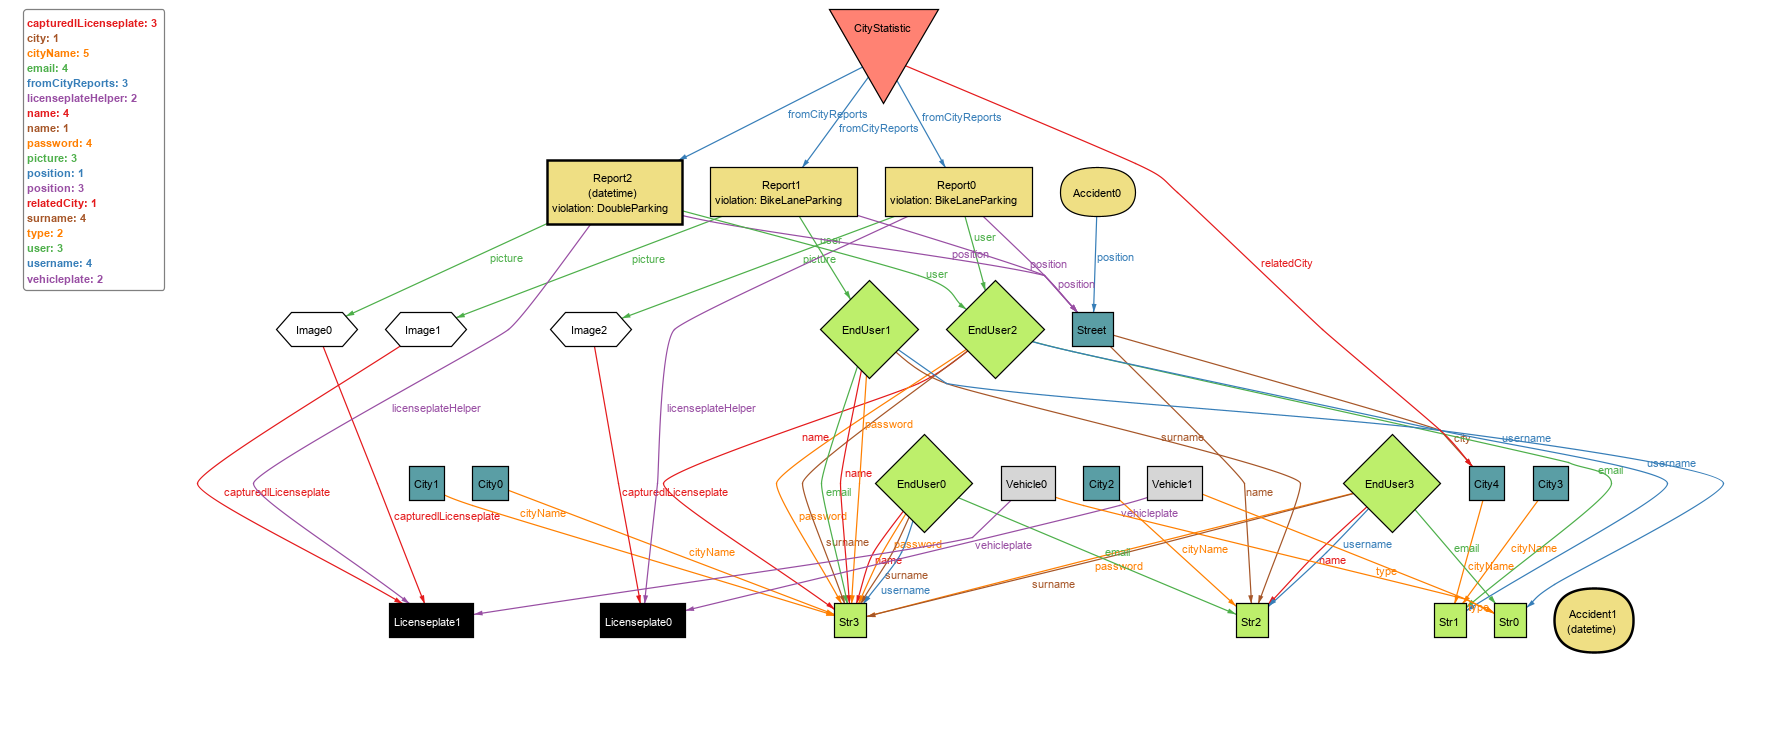
\includegraphics[width=1.1\linewidth, height=0.55\textheight]{Images/Alloy/world3alloy}
	\caption{World 3}
	\label{World3}
\end{figure}
